\chapter{Implementation of the System} \label{chap:implementation}

The chapter describes how the design of the system is implemented and the relevant challenges. Dedicated explanation of the technique specification can be found in this chapter as well. The key sequence diagrams are illustrated to brief the work flow of the system.

\section{Implementation on the Side of End Devices}

As mentioned in the chapter \ref{chap:design}, the end devices are simulated by android phones in my implementation. The target Internet of Things devices that play the role of sampling ambient information through a video format are assumed as weak computing devices. In other words, they follow the philosophy of design that more tasks are finished with less power and computing unit. The cost of them are low accordingly so that they are  realistic for large scale deployment.

\subsection{Android Devices}
Nexus6 is used in the experiment, which was published in 2014, about 4 years ago. This phone is manufactured by Motorola and embedded with a Qualcomm 2.7 GHz quad-core Krait 450 CPU.\cite{wiki:nexus6} The power of this android phone is not as strong as mainstream counterparts such as Google Pixel 2 nowadays. This weakness contributes to its competence as the replacement of devices in Internet of Things.

\subsection{Operating System}
The operating system version of this android phone is 7.1.1 "Nougat". API \cite{android-api} lever of this version is 15 while it is not compulsory since I just make use of the android.hardware.camera2 API that is introduced in Android 5.0 (API level 21).\cite{android5.0} This update enhances the control towards the camera so that fine-grain photos can be captured. 

\subsection{Image Capture}
The android phone is equipped with both front and rear camera. Only rear camera is used to capture the video stream. The resolution of the sensor is 13MP\cite{wiki:megapixel}, however, I do not extract image from camera directly, so the resolution do not decide the final size of the image.

The process of my sampling the images is as following. I make the application executed and turn the camera into preview mode in which camera continuously collect image frames and push to the surface view of the android application. Then another thread in the application manage to sample images from these surface view according to the frequency appointed. As a result, the resolution of the image is decided by the size of the screen which is about 2560 x 1440 px. The frequency is adjustable according to the configuration.

The preview images will be compressed with PNG format\cite{roelofs1999png} which is a loss-less image compression format with  broad compatibility among Internet . The quality level of image is set to 90 percent while the original image is reduced to half size. This help to decrease the pressure of network bandwidth.

\section{Network between End Devices and Fog Nodes}
In the previous part, the process of image collection is described. Since the face detection and recognition tasks are not arranged locally, they are assigned to the closest Fog Nodes.

The IP address of the Fog Node is hard coded into the application so rigid network configuration should be followed to make the application manage to locate the corresponding Fog Nodes. Dynamic Host Configuration Protocol (DHCP)\cite{droms2002dhcp} is an ideal protocol to handle the gap and actually it is used in my experiment .

An appointed IP address is remained for Fog Node deployment in every sub-network where Fog Node should be accessible. As the diagram \ref{fig:network} shows, end devices are connected to the Fog Nodes directly, within 1 hop ideally. The links between the Fog Node and Cloud Nodes in different sub networks(dyed in four different colours) are various. This uncertainty contributes to the network latency in part.

\section{Communication between End Devices and Fog Nodes}
The network part shares the underlying physical implementation of the system and this section covers the protocol used to transmit the collected image data to the Fog Nodes.

Consider Fog Nodes will be distributed into heterogeneous network, compatibility of the protocol owns a high priority. Hypertext Transfer Protocol(HTTP) is among main stream standards and play the role of De facto foundation for the World Wide Web \cite{fielding1999hypertext}. So I appoint it as the fundamental protocol for the application layer in the Internet protocol suite, namely TCP/IP.

Two-way communication is suitable for our scenario. Schedulers sample images and send them to the Fog Nodes for face identification in a recurring way. The instant outcomes will be pushed back to original devices as soon as possible. The data flow of processes mentioned above go in opposite direction, reveal the feature of two-way communication. So the traditional request-response client-server protocol is wiped out from the options due to its disqualification.

The frequency of requests also damage the shine of the HTTP because of its tedious handshake stage. Even though HTTP/1.1 introduced a keep-alive-mechanism to reuse the previous connection for the coming request, I prefer the emerging standard of full-duplex communication through HTTP.

WebSocket is favourable protocol that supports two-way communication and removes the dependence upon multiple HTTP connections\cite{fette2011websocket}. This mechanism is initially designed for carrying short message between clients(mainly browsers) between servers. It sounds marvellous for building a real-time chat channel, especially when it comes to compatibility. WebSocket integrates itself with HTTP protocol and is built with TCP. The default port of it is 80, which add on its highlights.\cite{fette2011websocket}

According to the characteristic of WebSocket mentioned, pre-processing of the images is invoked. Consider encoding schemes supported by HTTP, plain byte code should be converted before they are put into the payload. Base64 is made use of to avoid the omission of the data.

Base64 make underlying data can be delivered in a textual format to bypass certain legacy system or lead to better interoperability \cite{josefsson2006base16}. In our case, it is needed to encode binary data before it is transported to the server side to keep the data intact. The code section in the figure \ref{fig:png_base64} displays how I do the image pre-processing through the Java SDK.

\begin{figure}
    \centering
    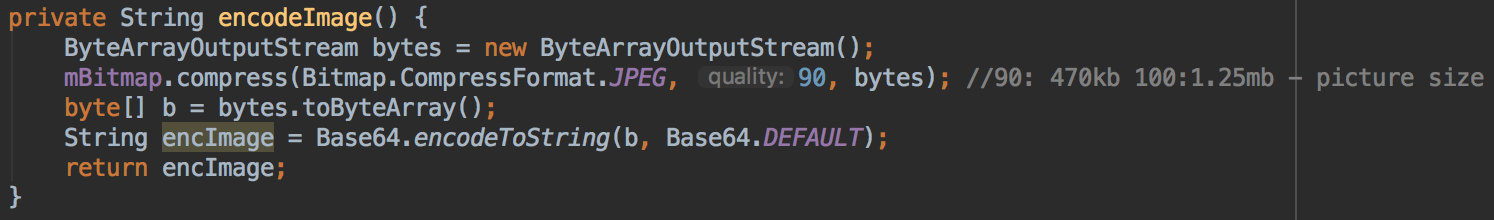
\includegraphics[width=\textwidth]{images/png&base64.png}
    \caption{Image Compress  Base64}
    \label{fig:png_base64}
\end{figure}



\begin{figure}
    \centering
    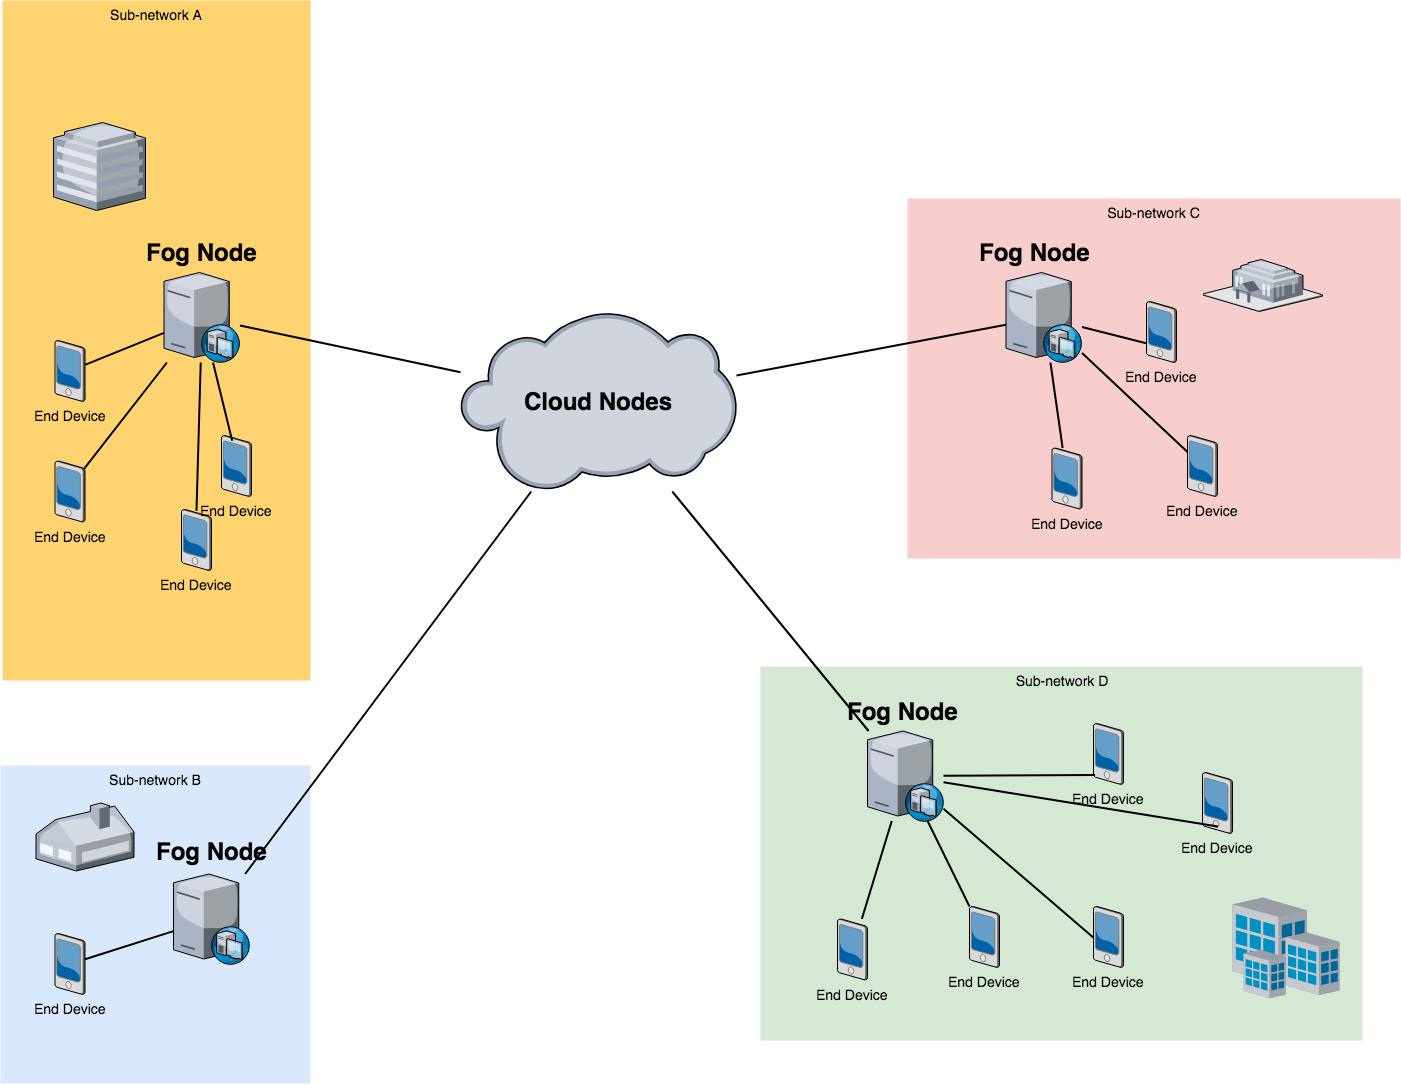
\includegraphics[width=\textwidth]{images/network.png}
    \caption{Network connection}
    \label{fig:network}
\end{figure}


\section{Implementation on the Side of Fog Nodes}
This section discusses the technical specification when it comes to build the corresponding Fog Nodes. The image pre-processing and data decoding processing are symmetric to the original one, so descriptions are briefed. Generally speaking, the images restore on the side of Fog Nodes and WebSockets keep consume incoming event with the payload of image and respond accordingly.

The following subsections focus on two routines implemented for performance benchmarks. The difference between them are algorithm of face identification.

\subsection{Fog Basic}
As displayed in the figure of \ref{fig:preview}, there is an button, the third button from the left, in charge of starting the mode of "Fog Basic". In this mode, the face identification tasks will be sent to the port on the server with the basic face detection functionality. 

\subsubsection{Face Detection}
OpenCV provides solid face detection module called Haar Feature-based Cascade Classifiers\cite{opencv_library}. In their tutorial documentation, they underline that this classifier is an effective object detection method. This method is proposed by Paul Viola and Michael Jones and depicted as a machine learning based algorithm \cite{viola2001rapid}. The algorithm extract features from the grey image and applies Adaboost to the virtually 160000+ features. Their paper argues 200 features offer the detection with 95\% accuracy. To improve the computing, a idea of discarding regions without face as early as possible is composed. This is the story behind classify the algorithm into Cascade of Classifiers.

To use Haar Feature-based Cascade Classifiers in my implementation, training stage can be saved due to existing trained model for human faces and eyes. The XML classifier file can be found in their SDK under the name of "haarcascade\_frontalface\_default.xml".

To stream images decoded from the end devices to the face detection module, OpenCV image manipulation module is introduced. The relevant operations include recognising the compression format of the image, extracting RGB information from the image container and map the RGB colour space to the Grey space. Because colour meta data is unnecessary to Haar algorithm, grey images are prerequisite of this algorithm.

Node-opencv provides the OpenCV bindings for Node.js\cite{node-opencv}. This third-party open source project is relied on to make the image stream interplay-able with the underlying native computing layer, namely OpenCV c++ native code.

\subsubsection{Web Server}
As discussed in the Communication section, WebSockets protocol is in use. Since it is just a protocol, it should be implemented by certain programming language or specific framework. This section offer detail about the required web application container or environment. 

Node.js is asynchronous event driven JavaScript runtime targeting at scalable network applications\cite{nodejs}. In their official documentation, Node.js regards HTTP as a first class citizen which means it put streaming and low latency in heart. The predominant advantages of Node.js make itself an appropriate candidate when it comes to implement WebSockets.

Among popular Github open source projects, Socket.io are gaining increasing popularity. This library features the fastest and most reliable real-time engine\cite{socketio}. It completely realise the standard of WebSockets and successfully build the rich ecosystem around it. SDK offered range from browser environment to cross platform mobile operation system such Android and iOS. Since its feature satisfied the requirement, it is used for Fog Basic mode as the middle-ware of the Web Server, running upon the Node.js runtime.

The node-opencv can be chained with the event handler of Socket.io, leading to saved context change and fewer data exchanges. Image data from end devices is collected and merged through Socket.io and handed over to the node-opencv simultaneously on the same Node.js runtime. 

\subsection{Fog DNN}
The button labelled with "Fog DNN" triggers another mode where deep learning based face recognition is used. You can see the button is located at the bottom centre of the figure \ref{fig:preview}.
The face identification algorithm compute the name of detected faces, other than just the location of the faces.  

\subsubsection{Face Recognition}
Compared to the prior mode of "Fog Basic", higher quality face identification tasks succeed in this mode. To be more specific, The Fog Basic mode only detects the location of the faces upon one image frame, while Fog DNN mode steps further. Fog DNN manage to compare faces to known faces to report the name of that face.

The functionality of face recognition is delivered by Dlib. Dlib is developed by Davis King and start with the target of building a general purpose library in 2002\cite{dlib09}. Considering the popularity of machine learning, relevant tools are focused as well. Deep metric learning tooling is added to the Dlib in recent releases.

Davis King, the contributor of the Dlib, implemented the ResNet network and imported it into the library last year. This model is an essential version of ResNet-34 network which is proposed through the paper Deep Residual Learning for Image Recognition\cite{he2016deep}. The model was reported to reach the accuracy of 99.38\% whose record can be found on the Labeled Faces in the Wild benchmark.

A python wrapper is developed by Adam Geitgey to bridge gap between python and C++\cite{python-facerecognition}. His library is relied on to implement my system.

\subsubsection{Web Server}
Since end devices connect to the server side through the protocol of WebSocket, face recognition algorithm cannot work only without the underlying web server. Given high demand of concurrency and leverage event driven pattern similar to Node.js, AIOHTTP is used to offer the asynchronous capability \cite{python-aiohttp}.

I also rely asyncio to write single-thread concurrent code with coroutines, multiplexing I/O because the native I/O in python is blocking and operate awkwardly with AIOHTTP. 

\section{Implementation on the Side of Cloud Nodes}
The Cloud Nodes almost share the same code with Fog Nodes with Fog DNN mode. The Cloud Nodes can be regards as an elastic resource pool. When the amount of the requests soars beyond the capability of assigned Fog Node, the request will be redirected to Cloud Nodes. The Fog Node that fails to handle the request looks like a proxy.

The decision of whether the computing should happen on Fog Nodes and Cloud Nodes is dependant on the dynamic allocation algorithm deployed on Fog Nodes.

\subsection{Fog Cloud}
Fog Cloud mode can be activated through the button in the figure \ref{fig:preview} with the same name. In this mode, requests from the end devices are doubled or tripled to mimic the situation where Fog Nodes themselves are unbearable to respond to end devices and quality of service is damaged. In that case, Cloud infrastructures participate the system to handle the requests handed over from Fog Nodes.

As presented, the code repository of the Cloud Nodes is quite similar to the counterpart in Fog Nodes with DNN mode. Normally, Cloud Nodes are elastic enough to be regraded as infinite computing source. So Basic mode is not implemented at all in the cloud.

The difference between Fog Nodes with DNN mode and Cloud Nodes exists on the deployment. Code on the cloud is executed on the Amazon EC2 instances and embrace the concept of server-less. As a result, if the tasks surge upwards, they can scale up transparently. On the contrary, the deployment of Fog Nodes is solid in that case, the hardware is fixed even though there are a large number of request.

\subsection{Dynamic Allocation Algorithm}
Dynamic allocation algorithm plays the role of traffic controller when it comes to decide the location of computing tasks. The core of the algorithm is to calculate whether the assigned Fog Node owns the competence of maintain expected quality of service and if not, how many extra computing units are in need.

The mechanism can be explained as follows. There are monitors running in the Fog Nodes. These monitors record the number of the requests(N) for the previous second. The computing time slots(T) are also recorded for every request. Then mathematical expectation of the computing time slot can be calculated based on the data, called(ET). Then I assume the coming second holds the same number of requests(N). The assumed {TODO!!!}

\section{Response Data Optimisation}
To reduce the amount of the data transferred from the Fog Nodes or Cloud Nodes, only coordinate and face related meta-data are return. The outcome are combined in the end devices. In other word, android devices receive these data and visualise it based on preview frame to make the process look like real-time. Originally, the image with detection frames within it will be returned from the Fog Nodes or Cloud Nodes directly. 

\section{Controlled Experiment Setting}
In order to make the performance of Fog Computing based face identification more impressive, two parallel experiments are introduced. These modes involve no Computing units outside the end devices.

\subsection{Native Mode}
Native mode makes the face detection algorithm happen on native layer of the android system. The architecture of the Android System can be found in the figure of \ref{fig:android_application_layer}.

Android applications run on ART or its predecessor Dalvik which are runtime for Dex bytecode files\cite{android-art}. The code invoking camera works on the native layer of the Android System. The memory of executables cannot be shared directly if they are allocated to different layers. The JNI helps to transmit data between native layer(orange part) and application layer(green part).

In the native mode, I chain the face detection task after the image capture and paint the outcome upon the preview frame. As a result, the data of the image remains in the native layer without necessary of movement.


\begin{figure}
    \centering
    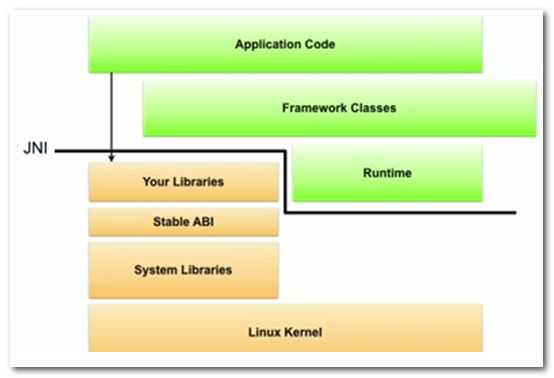
\includegraphics[width=\textwidth]{images/jni.jpg}
    \caption{Android Application Layer}
    \label{fig:android_application_layer}
\end{figure}

\subsection{Local Mode}
Even though the native mode reveal the performance of keeping the face detection in the low power end devices, the computing model is not universal. In other word, a more isolated model should be used to make it more convincing. For example, general computing task will be coded in the application layer with specific JVM supported programming languages such Java or Kotlin but in C++ which relies on NDK to manipulate the hardware. 

To expose the data to the application layer, migration of the data from native layer to application layer is unavoidable. This process can be found in local mode, where data is transferred to the application layer before the face detection is applied.

\section{Key Sequences Diagram}
After discussing the decomposed components of the system, blueprint of it can be view in key sequences diagrams.
The figure \ref{fig:off-peak_mode_sequence} and the figure \ref{fig:peak_mode_sequence} display the sequence diagram of the system. The first figure illustrates the sequence diagram for the off-peak mode and the following one expresses the logic of peak mode.

\subsection{Off-peak Mode Sequence}
As you can see in the figure of \ref{fig:off-peak_mode_sequence}, there are two lifelines, namely end-devices and Fog Nodes. The initial point locates at the left side of the diagram, which is the start point of the application.

The instruction above this point says "choose computing mode". The computing mode here refers to five modes inbuilt with the android application. These five sub-modes can be observed at the bottom of the figure of \ref{fig:preview}. They are discussed in the previous sections.

The loop of processes are summarised as follows (Fog Basic and Fog DNN modes only, Native and Local modes are excluded):
\begin{enumerate}
    \item capture previews from the camera
    \item compress and encode the image and send the data to the Fog Node
    \item Face Detection and Face Recognition according to the chosen mode
    \item Return data consist of locations of faces and related name meta-data
    \item Draw the frame on the end device
\end{enumerate}

\subsection{Peak Mode Sequence}
The figure of \ref{fig:peak_mode_sequence} displays the situation when Fog Cloud mode is activated. As the figure depicted, there extra one lifeline compared to off-peak mode sequence. The Cloud Nodes lifeline illustrate the functionality of the cloud computing infrastructure. The comment in the diagram points out the stage where dynamic allocation algorithm is taken in part.

the loop of processes are complemented as follows (Fog Cloud Mode):
\begin{enumerate}
    \item capture previews from the camera
    \item compress and encode the image and send the data to the Fog Node
    \item Decide the location of the face recognition task
    \item If bearable load, face recognition in the Fog Nodes
    \item If overload happens to the Fog Nodes, face recognition tasks are allocated to Cloud Nodes
    \item Return data consist of locations of faces and related name meta-data
    \item Draw the frame on the end device
\end{enumerate}

\begin{figure}
    \centering
    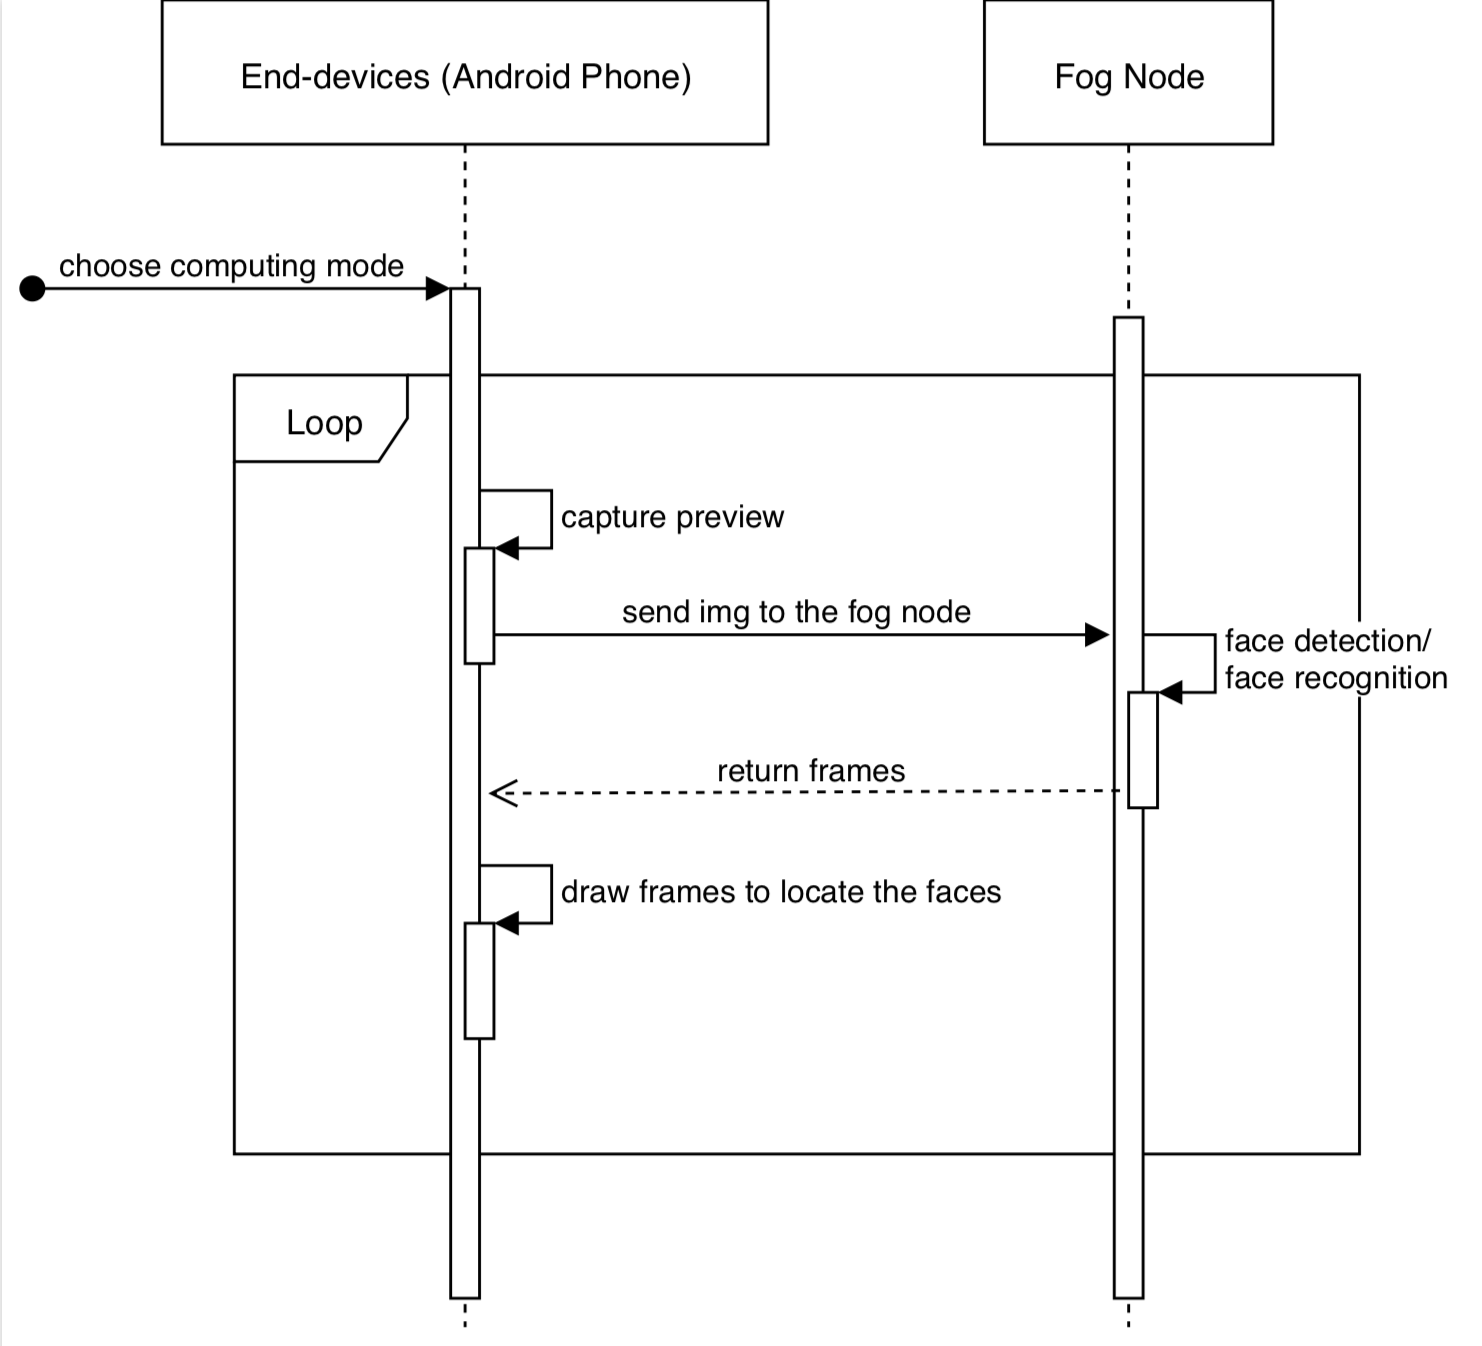
\includegraphics[width=\textwidth]{images/fog_mode.png}
    \caption{Off-peak Mode Sequence}
    \label{fig:off-peak_mode_sequence}
\end{figure}

\begin{figure}
    \centering
    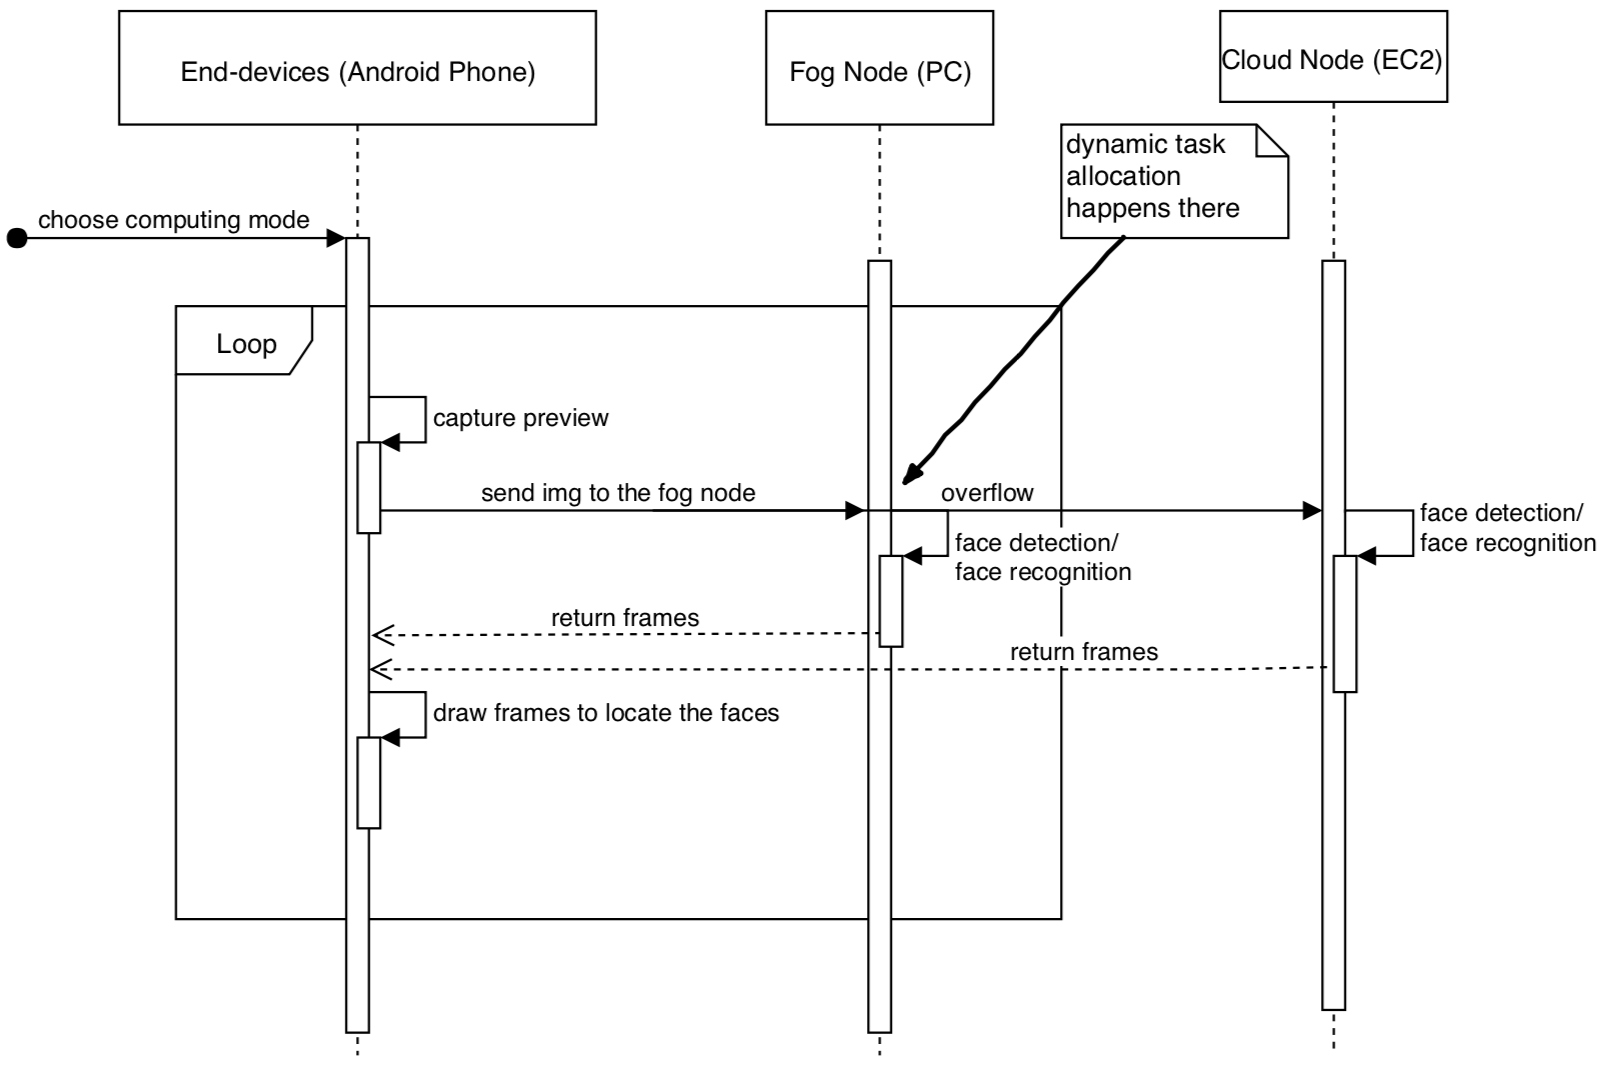
\includegraphics[width=\textwidth]{images/cloud_mode.png}
    \caption{Peak Mode Sequence}
    \label{fig:peak_mode_sequence}
\end{figure}


\begin{figure}
    \centering
    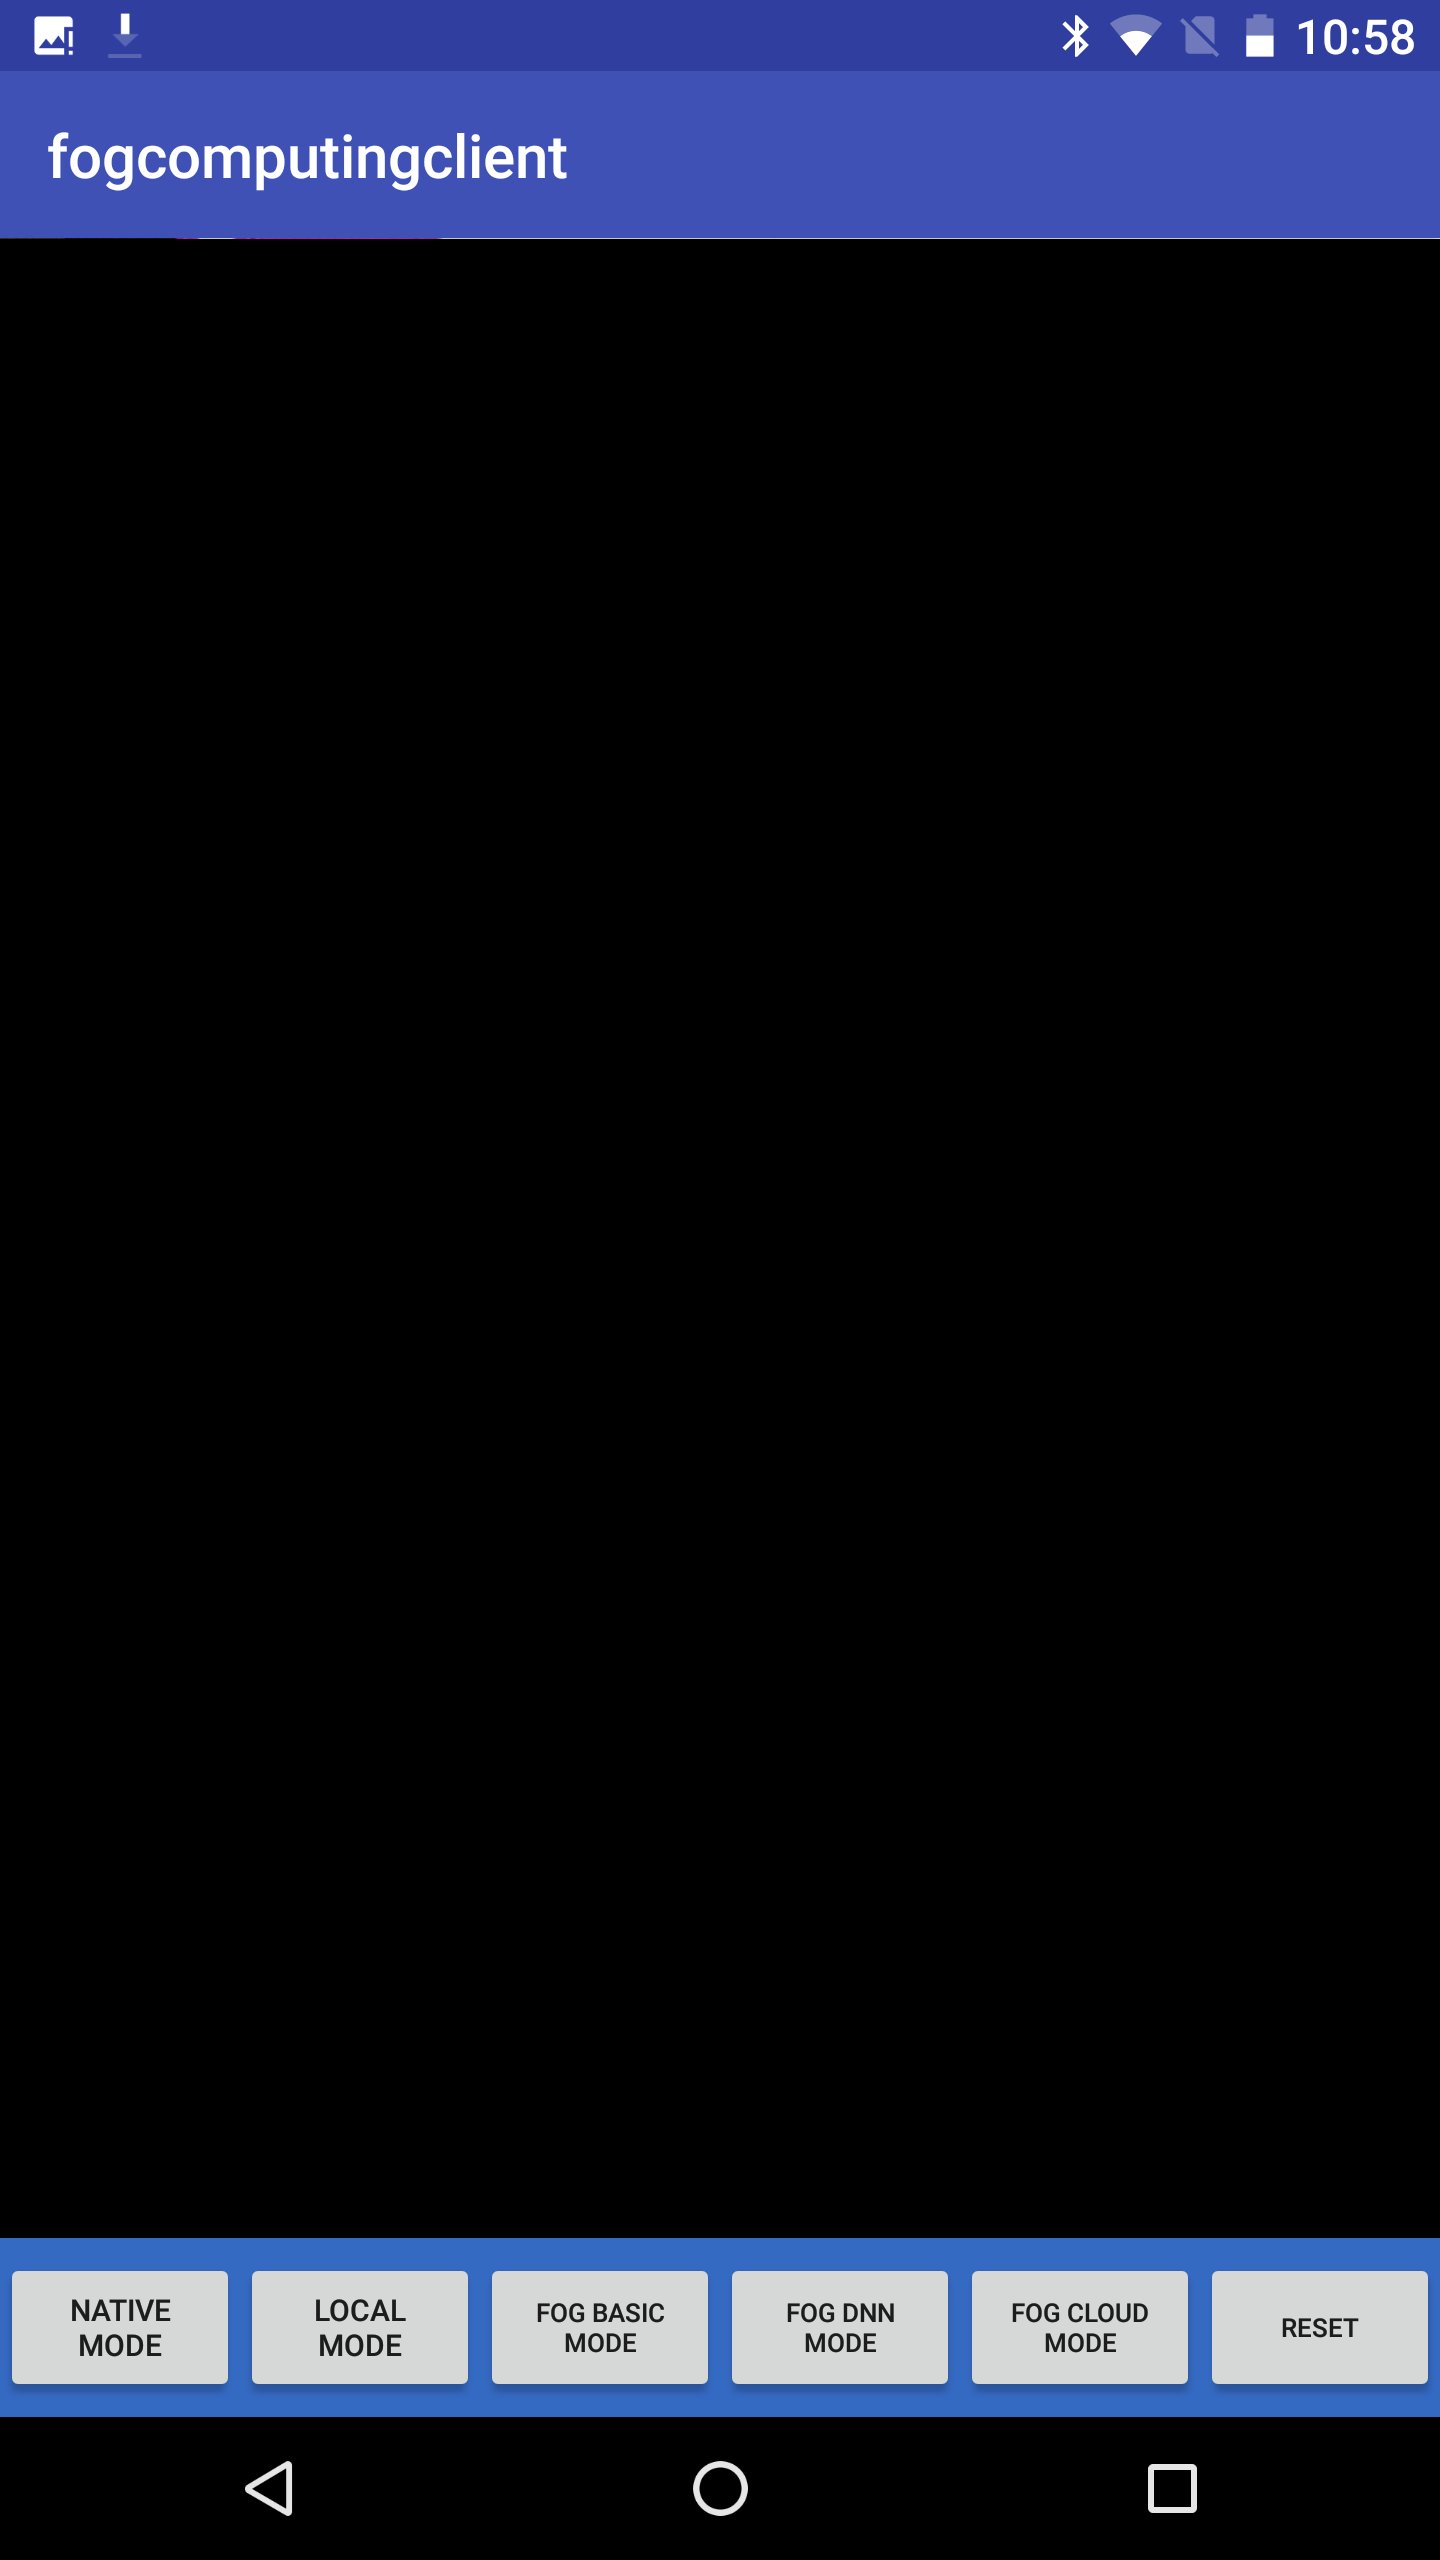
\includegraphics[width=0.5\textwidth]{images/preview.png}
    \caption{Preview of the End Devices(Android)}
    \label{fig:preview}
\end{figure}

